\section{The optimal setup}\label{sec:4:optimal-setup}
With the general framework in hand, the next logical question to ask is, if the stability against placement-variations can be improved.
The general rule of thumb for these optimizations is the following:
Increase the gravitational interaction by either heavier and larger particles or by reducing the separation distance $L$ without substantial sacrifices of experimental realization.
As an example, the stability increases intuitively by increasing the separation distance $L$. However, this does also increase the time $t_\mathrm{max}$ until the maximum amount of entanglement can be measured which would increase the total time  $\sim \# t_\mathrm{max}$ of the experiment with $\#$ individual measurements.
It is not immediately obvious, how the stability and the maximum possible variations $\Delta \theta_\mathrm{crit}$ and $\Delta L_\mathrm{crit}$ behave for the change in parameters.
In the following section, precisely the changing of this stability is discussed for changing the orientation $\alpha, \beta$, the separation $L$, the mass $M_A = M_B \equiv M$ and the superposition size $\Delta x_A = \Delta x_B \equiv \Delta x$.


\subsection{Orientation}
The arguably easiest parameter to change experimentally is the orientation of the superpositions relative quantified by $\alpha$ and $\beta$ in \cref{fig:4:complete-setup}.
As could be already seen in \cref{fig:2:entanglement-dynamics} in \cref{cha:first-look}, the entanglement dynamics are dependent on the orientation. 
The particles in the parallel orientation have to evolve twice as long compared to the orthogonal orientation to get maximally entangled.
In general, it is beneficial to aim for the highest entanglement rate and thus for the smallest $t_\mathrm{max}(\alpha, \beta)$ as this requires a smaller coherence time and the total experimental time can be reduced.
The earlier results from \cref{cha:first-look} can be more generalized for an arbitrary orientation $\alpha, \beta$. The logarithmic negativity is given by
\begin{equation}
  E_N = \log_2\left(1+\abs{\sin\Delta\phi}\right)
\end{equation}
where $\Delta\phi$ now depends on the orientation and is given by (for $\Delta x \ll L$)
\begin{equation}
  \Delta \phi = \frac{G M_A M_B t \Delta x_A \Delta x_B}{8\hbar L^3} \left(\sin\alpha\sin\beta-\frac{1}{2}\cos\alpha\cos\beta\right) .
\end{equation}
The maximum entanglement $E_N=1$ is reached for $\Delta\phi = \pm \pi/2$ and thus after a time
\begin{equation}\label{eq:4:t-max}
  t_\mathrm{max}(\alpha,\beta) = \frac{4\pi \hbar L^3}{G M_A M_B \Delta x_A \Delta x_B}\abs{\sin\alpha\sin\beta - \frac{1}{2}\cos\alpha\cos\beta}^{-1}.
\end{equation}
The resulting times are shown in \cref{fig:4:t-max-orientation}.
\begin{figure}[!htbp]
  \centering
  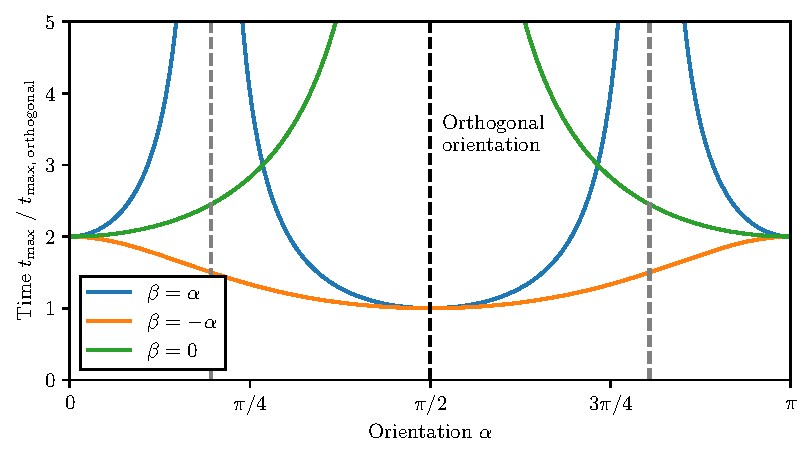
\includegraphics[width=\textwidth]{./../figures/ideal-entanglement/t-max-orientation.pdf}
  \caption{Time $t_\mathrm{max}$ after which maximum entanglement ($E_N = 1$) is reached for different orientations. Only the most interesting and highly symmetric cases $\alpha=\pm\beta$ and $\beta=0$ are shown.}
  \label{fig:4:t-max-orientation}
\end{figure}
The global minima of $t_\mathrm{max}(\alpha,\beta)$ is reached in the orthogonal orientation. This is not surprising considering that this orientation maximizes the difference in separation distance between all superposition states.
Much more interesting are the apparent singularities in \cref{fig:4:t-max-orientation} which arise for 
\begin{equation}
  \sin\alpha\sin\beta=\frac{1}{2}\cos\alpha\cos\beta .
\end{equation}
For $\beta=0$ the singularity for $\alpha=\pi/2$ is not surprising. In this configuration, the distances $\ket{\psi^1_A}\leftrightarrow\ket{\psi^{1,2}_B}$ and $\ket{\psi^2_A}\leftrightarrow\ket{\psi^{1,2}_B}$ are the same and thus these states accumulated the same phases, which results in a factorable global phase.
In the case of $\alpha=\beta$, the two singularities are precisely given in the orientation
\begin{equation}
  \alpha=\beta=2 \arctan(\sqrt{3}\pm\sqrt{2})\approx 90\deg \pm 54.74\deg .
\end{equation}
There does not exist a straight-forward geometric interpretation why no entanglement is generated in this configuration, however all 4 separation distances between the states precisely form the \q{harmonic mean} visualized in \cref{fig:4:harmonic-mean}.
\begin{figure}[!htbp]
  \centering
  \def\svgwidth{\textwidth}
  \input{./../figures/harmonic-mean.pdf_tex}
  \caption{\textbf{left:} The system in the orientation $\alpha=\beta=2\arctan(\sqrt{3}-\sqrt{2})$. For $\Delta x \ll L$, ll separation distances exactly lie in the \textit{harmonic mean}. \textbf{right:} Geometric visualization of the harmonic mean.}
  \label{fig:4:harmonic-mean}
  % COLORFUL:: $\textcolor[HTML]{aa0000}{\blacksquare} = \displaystyle\frac{2}{\frac{1}{\textcolor[HTML]{0044aa}{\blacksquare}}+\frac{1}{\textcolor[HTML]{447821}{\blacksquare}}}$
\end{figure}
To avoid all these singularities, it is advisable to always take $\alpha=-\beta$, where all orientations result in roughly similar entanglement times, at most only differing by a factor of $2$.

It should come by no surprise that the different orientations exhibit different stabilities. Logically, one would expects that the orthogonal configuration is much more sensitive against angular variations compared to the parallel one.
On the contrary, the parallel configuration should be much more stable against variations in the distance, as no phase difference (\q{dephasing}) between the two superposition states $\ket{\psi^1_{A(B)}}$ and $\ket{\psi^2_{A(B)}}$ of the same mass is induced.

The effect of different orientations on the stability against angular variations and how the critical angular variation $\Delta \theta_\mathrm{crit}$ behaves is shown in \cref{fig:4:theta-crit-orientation}.
\begin{figure}[!htbp]
  \centering
  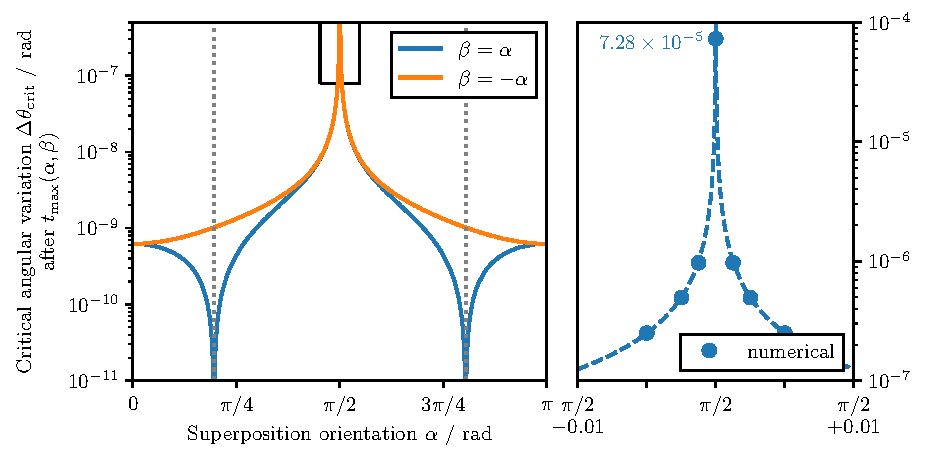
\includegraphics[width=0.95\textwidth]{./../figures/theta-variance/theta-crit-orientation-complete.pdf}
  \caption{Maximum possible allowed angular variation $\Delta\theta_\mathrm{crit}$ for different orientations. All data-points where calculated at the time of maximum entanglement shown in \cref{fig:4:t-max-orientation}. The \emph{orthogonal configuration} is very stable against angular disturbances. At $\alpha=\beta=\pi/2$, only exact numerical results show a finite value. The singularities on the left figure arise from the fact, that these configurations need infinite time to entangle as already seen in \cref{fig:4:t-max-orientation}.}
  \label{fig:4:theta-crit-orientation}
\end{figure}
As expected, the orthogonal configuration is the most stable against these kind of variations. This is, because the dephasing ultimately depends on the distance between the state and the shield $L \pm \Delta x/2 \cos\theta \approx L \pm \Delta x/2 (1 - \theta^2/2)$, which is a only second order effect of the angular variations $\theta$.
This explains the apparent \q{infinitely} good stability in the figure, as the analytical solution only uses first order approximations in $\theta$.
Exact numerical results however cap the stability at $\Delta \theta_\mathrm{crit,\,orthogonal} \approx 7.3\times 10^{-5}\si{rad}$.

Respectively, the stability against distance variations $\Delta L_\mathrm{crit}$ for different orientations is shown in \cref{fig:4:L-crit-orientation}.
\begin{figure}[!htbp]
  \centering
  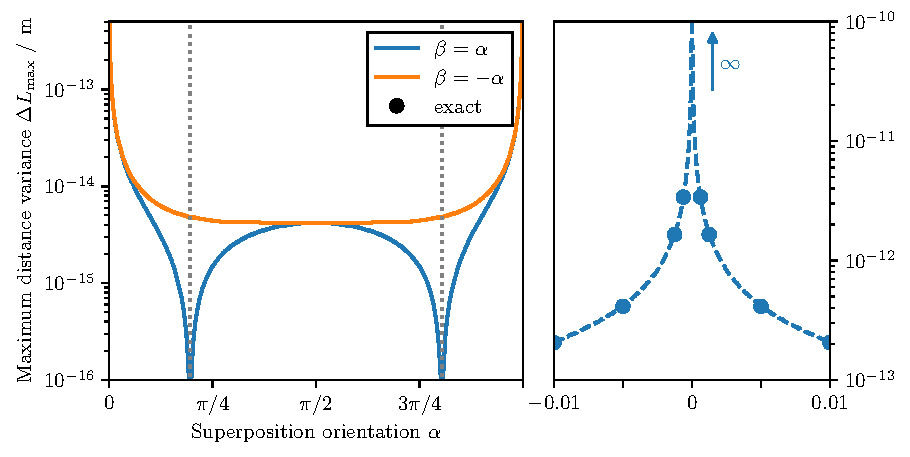
\includegraphics[width=0.95\textwidth]{./../figures/L-variance/L-max-orientation-complete.pdf}
  \caption{Maximum possible allowed distance variation $\Delta L_\mathrm{crit}$ for different orientations. This figure is similar to \cref{fig:4:theta-crit-orientation}, only for distance variations. On the contrary to angular variations, the \emph{parallel configuration} is infinitely stable against changes in the distance between the shield and the cat-state.}
  \label{fig:4:L-crit-orientation}
\end{figure}
Again aligning with expectations, the parallel configuration is (in theory) exhibits an infinite stability.
One however could argue, that a for this to hold, the uncertainties in the angular placement have to be zero. As could be seen in \cref{fig:4:theta-crit-orientation}, these variations are at most around $\sim 5 \times 10^{-5}\si{rad}$ and thus a realistic upper bound for the minimum required distance variations is given by $\Delta L_\mathrm{crit,parallel} \simeq 4\times 10^{-11}\si{m}$.
It is important to keep in mind, that these stability values can be improved substantially by changing e.g. the separation distance $L$ or the particle size $R$.

Looking at these results, the parallel orientation seems like the only realistic experimental option even though it requires lager coherence times $t_\mathrm{max}$.
Keeping separation variations below $0.01\si{nm}$ - roughly the size of a single atom - is virtually impossible considering thermal vibrations of the shield and the sphere cannot be fully prevented and are in the same order of magnitude, as seen later in \cref{cha:the-shield}.
With this data on hand, it is possible to construct a stability diagram \cref{fig:4:optimal-orientation}, showing the ideal orientation in which the most entanglement can be measured.
\begin{figure}[!htbp]
  \centering
  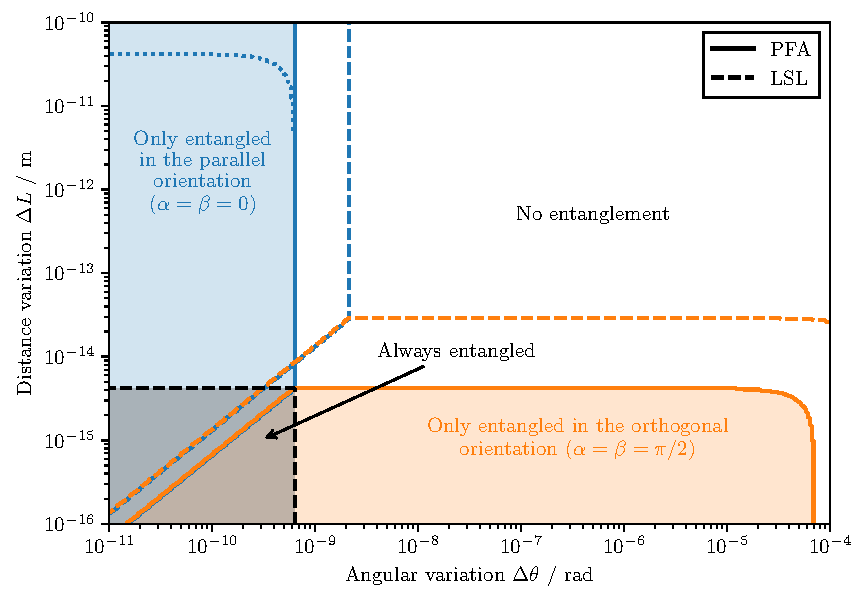
\includegraphics[width=\textwidth]{./../figures/optimize/optimized-orientation-advanced.pdf}
  \caption{Optimal orientation for the experimental setup dependent on the variations in angle $\Delta\theta$ and distance $\Delta L$ for a initial separation distance of $L=2R=2\times 10^{-5}\si{m}$ at time $t_\mathrm{max}$. The different predictions for the proximity-force-approximation (PFA) and the large-separation-limit (LSL) are shown. At distance $L=20\si{\mu m}$ the actual casimir interaction is somewhere in the middle between both approximation methods. In the region where entanglement is given regardless of the orientation (the bottom left), the orientation with \textit{more} entanglement is still colored. The dotted line corresponds to the realistic upper bound discussed in the text.}
  \label{fig:4:optimal-orientation}
\end{figure}
For most of the regions in the diagram, entanglement is only given in one certain orientation.


\subsection{Separation, mass and superposition size}

\begin{figure}[!htbp]
  \centering
  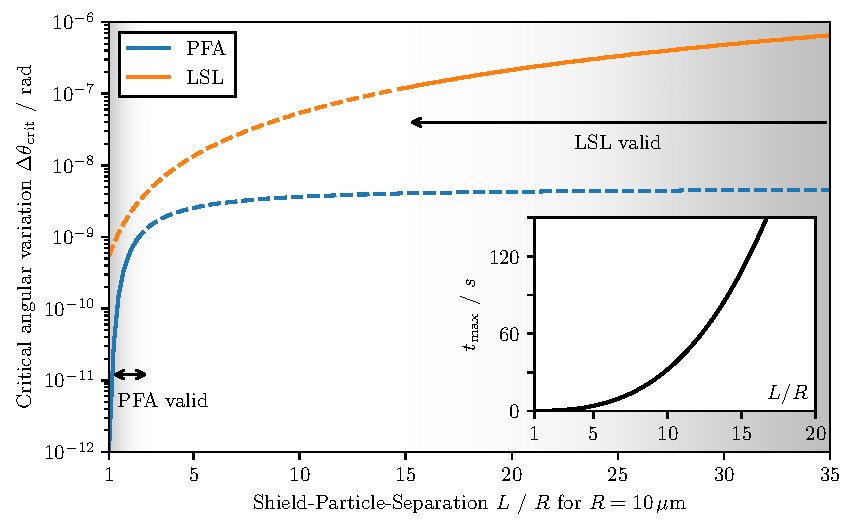
\includegraphics[width=\textwidth]{./../figures/theta-variance/theta-crit-L.pdf}
  \caption{R is fixed as $R=10^{-5}\si{m}$}
  \label{fig:4:theta-crit-L}
\end{figure}

\begin{figure}[!htbp]
  \centering
  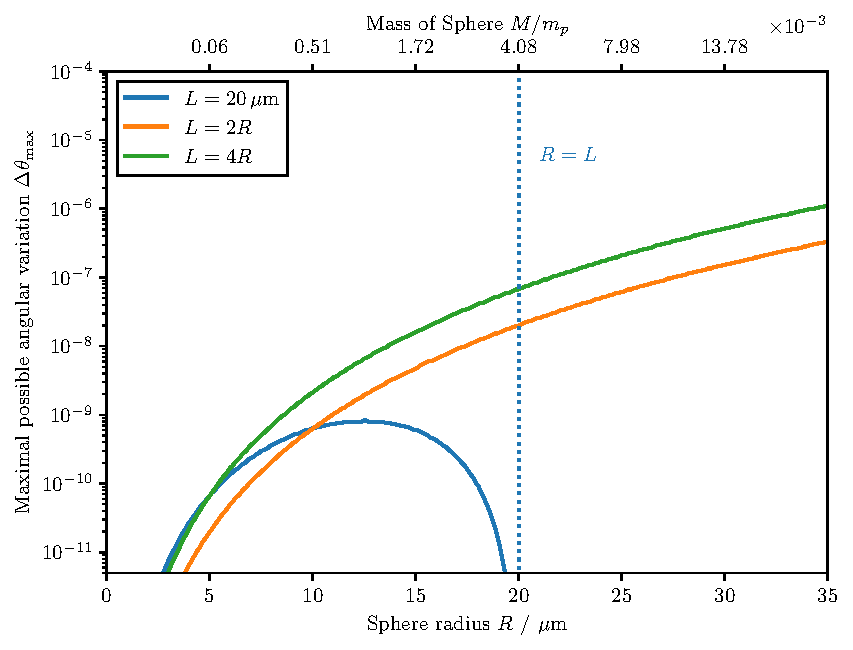
\includegraphics[width=\textwidth]{./../figures/theta-variance/theta-max-mass.pdf}
  \caption{...}
  \label{fig:4:theta-crit-mass}
\end{figure}

\begin{figure}[!htbp]
  \centering
  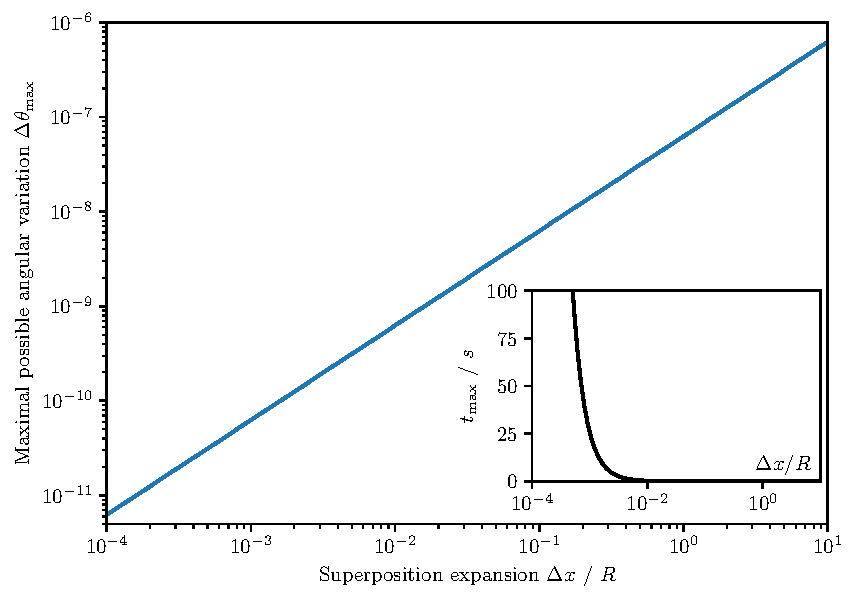
\includegraphics[width=\textwidth]{./../figures/theta-variance/theta-max-superpos-extension.pdf}
  \caption{...}
  \label{fig:4:theta-crit-superposition-size}
\end{figure}



% % \section{Stability in different orientations}\label{sec:4:orientation}
As could be already seen in \cref{fig:2:entanglement-dynamics} in \cref{cha:first-look}, the entanglement dynamics and especially the time $t_\mathrm{max}$ of maximum entanglement highly depend on the orientation.
There, it was shown already, that the for the parallel configuration the maximum entanglement is reached twice as slow as in the orthogonal orientation.
This result can be more generalized for an arbitrary orientation quantified by $\alpha$ and $\beta$ from \cref{fig:4:complete-setup}.


\begin{equation}
  E_N = \log_2\left(1 + \abs{\sin\Delta \phi}\right)
\end{equation}
where $\Delta \phi$ is now dependent on the orientation and is given by (for $\Delta x \ll L$)
\begin{equation}
  \Delta \phi = \frac{G M_A M_B t}{\hbar}\frac{\Delta x_A \Delta x_B}{8 L^3} \left[\sin\alpha\sin\beta - \frac{1}{2}\cos\alpha\cos\beta\right] .
\end{equation}
The maximum entanglement is again reached after $\Delta\phi = \pi/2$ and thus is also dependent on the orientation
\begin{equation}\label{eq:4:t-max}
  t_\mathrm{max} = \frac{4\pi L^3\hbar}{GM_AM_B\Delta x_A \Delta x_B} \abs{\sin\alpha\sin\beta - \frac{1}{2}\cos\alpha\cos\beta}^{-1}.
\end{equation}
The resulting times are shown in \cref{fig:4:t-max-orientation} and align with earlier results for the special cases of the orthogonal and parallel configuration.
\begin{figure}[!htbp]
  \centering
  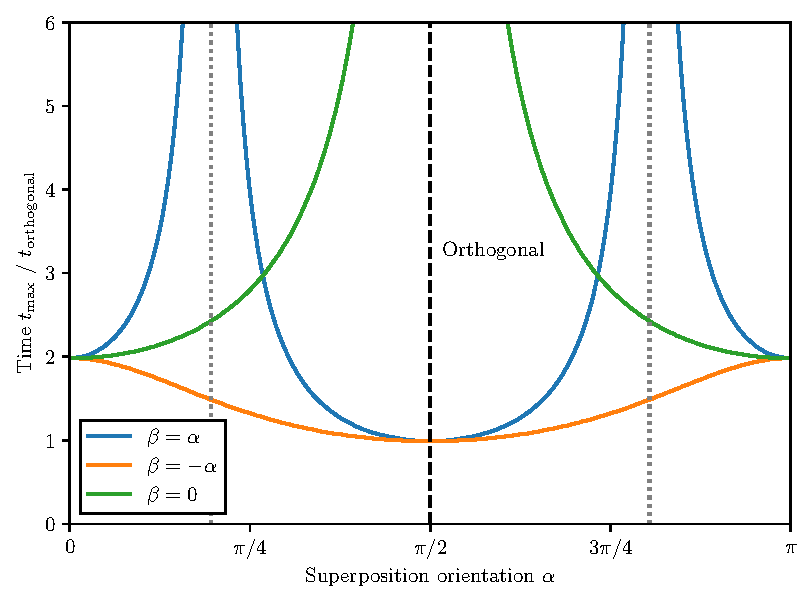
\includegraphics[width=\textwidth]{./../figures/ideal-entanglement/EN-orientation.pdf}
  \caption{Time of maximum entanglement $t_\mathrm{max}$ relative to $t_\mathrm{max,orthogonal}$ of the orthogonal configuration for different orientations. Some orientations like $\alpha=\pi/2$ and $\beta=0$ cannot induce any entanglement at all because of symmetry considerations.}
  \label{fig:4:t-max-orientation}
\end{figure}
The global minima of $t_\mathrm{max}$ is given in the orthogonal configuration meaning that of all possible configurations, this one induces entanglement the fastest. Considering the discussions in the end of \cref{cha:first-look}, this is not very surprising.
Much more interesting are the apparent singularities which arise for 
\begin{equation}
  \sin\alpha\sin\beta = \frac{1}{2}\cos\alpha\cos\beta .
\end{equation}
For $\beta=0$, the singularity in $t_\mathrm{max}$ at $\alpha=\pi/2$ is not surprising. At this configuration, the distances $\ket{\psi_A^1} \leftrightarrow \ket{\psi_B^{1,2}}$ are identical as well as $\ket{\psi_A^2} \leftrightarrow \ket{\psi_B^{1,2}}$. 
For the case $\alpha = \beta$, the two singularities are precisely given at
\begin{equation}
  \alpha = \beta = 2\arctan(\sqrt{3}\pm\sqrt{2}) \approx 90\deg \pm 54.74\deg.
\end{equation}
There does not exist a clear geometric explanation why no entanglement is generated in this configuration, however, all distances between the superpositions for a harmonic mean as visualized in \cref{fig:4:harmonic-mean}.
\begin{figure}[!htbp]
  \centering
  \def\svgwidth{\textwidth}
  \input{./../figures/harmonic-mean.pdf_tex}
  \caption{\textbf{left:} Arrangement in the orientation $\alpha=\beta=2\arctan(\sqrt{3}-\sqrt{2})$. All distances exactly lie in the \textit{harmonic mean} (for $\Delta x \ll L$). \textbf{right:} Geometric visualization of the harmonic mean.}
  \label{fig:4:harmonic-mean}
  % COLORFUL:: $\textcolor[HTML]{aa0000}{\blacksquare} = \displaystyle\frac{2}{\frac{1}{\textcolor[HTML]{0044aa}{\blacksquare}}+\frac{1}{\textcolor[HTML]{447821}{\blacksquare}}}$
\end{figure}





\begin{figure}[!htbp]
  \centering
  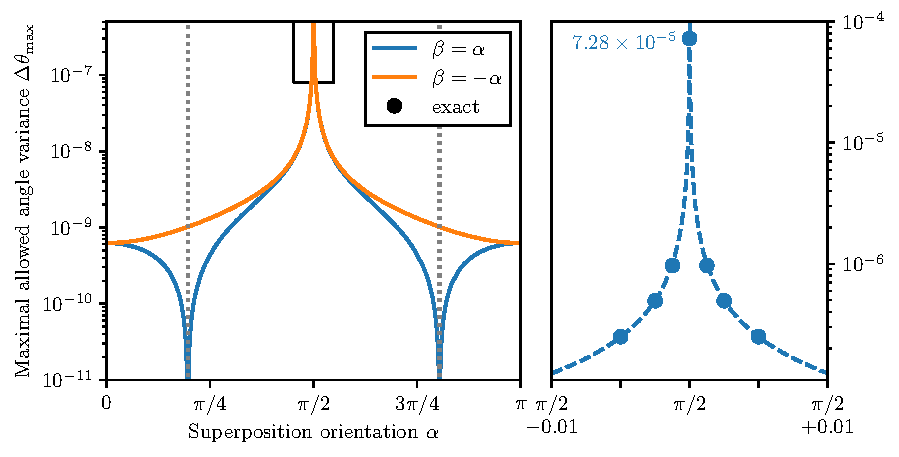
\includegraphics[width=0.95\textwidth]{./../figures/theta-variance/theta-max-orientation-complete.pdf}
  \caption{Maximum possible allowed angular variation $\Delta\theta_\mathrm{max}$ for different orientations. All data-points where calculated at the time of maximum entanglement shown in \cref{fig:4:t-max-orientation}. The \emph{orthogonal configuration} is very stable against angular disturbances. At $\alpha=\beta=\pi/2$, only exact numerical results show a finite value. The singularities on the left figure arise from the fact, that these configurations need infinite time to entangle as already seen in \cref{fig:4:t-max-orientation}.}
  \label{fig:4:theta-max-orientation}
\end{figure}

\begin{figure}[!htbp]
  \centering
  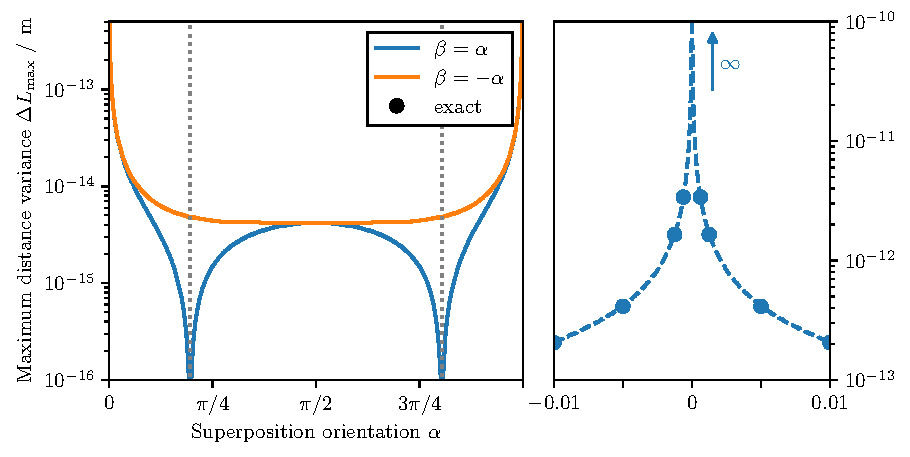
\includegraphics[width=0.95\textwidth]{./../figures/L-variance/L-max-orientation-complete.pdf}
  \caption{Maximum possible allowed distance variation $\Delta L_\mathrm{max}$ for different orientations. This figure is similar to \cref{fig:4:theta-max-orientation}, only for distance variations. On the contrary to angular variations, the \emph{parallel configuration} is infinitely stable against changes in the distance between the shield and the cat-state.}
  \label{fig:4:L-max-orientation}
\end{figure}



\begin{figure}[!htbp]
  \centering
  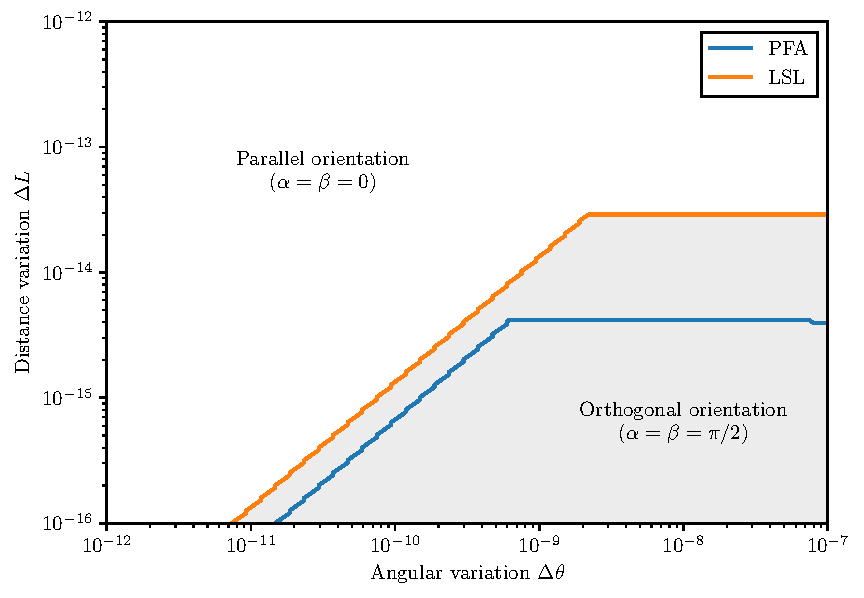
\includegraphics[width=\textwidth]{./../figures/optimize/optimized-orientation.pdf}
  \caption{Optimal orientation for arbitrary variations in the angle $\Delta\theta$ and the distance $\Delta L$. The optimum was calculated for different models of the Casimir-interaction (PFA eq. \eqref{eq:3:PFA-sphere-plate} and LSL eq. \eqref{eq:3:casimir-sphere-plate}).If angular variations dominate, the orthogonal configuration is best, whereas for large distance variations, a parallel orientation is advised.}
  \label{fig:4:optimal-orientation}
\end{figure}
